% Paquets généraux
\documentclass[a4paper,12pt,titlepage]{article}
\usepackage[T1]{fontenc}
\usepackage[utf8]{inputenc}
\usepackage[french]{babel}
\usepackage[gen]{eurosym}
%\usepackage[dvips]{graphicx}
\usepackage{fancyhdr}
\usepackage{pdfpages} 
\usepackage{multido}
\usepackage{hyperref}
%\usepackage{textcomp}
%\usepackage{aeguill}
\usepackage{schemabloc}
\usepackage[bitstream-charter]{mathdesign}
\usepackage{minted}

\newcommand{\id}{71}
\newcommand{\nom}{Théorie des mécanismes}
\newcommand{\sequence}{04}
\newcommand{\nomsequence}{Liaisons entre les solides}
\newcommand{\num}{02}
\newcommand{\type}{KH}
\newcommand{\descrip}{Liaisons équivalentes, hyperstatisme, liaisons en série et en parallèle, théorie des graphes}
\newcommand{\competences}{B2-12: Proposer une modélisation des liaisons avec leurs caractéristiques géométriques. \\ &  B2-13: Proposer un modèle cinématique paramétré à partir d'un système réel, d'une maquette numérique ou d'u \\ &  B2-17: Simplifier un modèle de mécanisme. \\ &  B2-18: Modifier un modèle pour le rendre isostatique. \\ &  C1-04: Proposer une démarche permettant d'obtenir une loi entrée-sortie géométrique.  \\ &  C2-05: Caractériser le mouvement d'un repère par rapport à un autre repère. \\ &  C2-06: Déterminer les relations entre les grandeurs géométriques ou cinématiques. }
\newcommand{\nbcomp}{7}
\newcommand{\systemes}{}
\newcommand{\systemesnum}{}
\newcommand{\systemessansaccent}{}
\newcommand{\ilot}{2}
\newcommand{\ilotstr}{02}
\newcommand{\dossierilot}{\detokenize{Ilot_02 }}


\newcommand{\auteurun}{Renaud Costadoat}
\newcommand{\auteurdeux}{Françoise Puig}
\newcommand{\institute}{Lycée Dorian}


\usepackage{color}
\usepackage{xcolor}
\usepackage{colortbl}
\usepackage{helvet}
\usepackage[frenchmath]{newtxsf} % for sans serif symbols
\renewcommand{\familydefault}{\sfdefault}
%\usepackage{amsfonts}
%\usepackage{amsmath}
%\usepackage{lmodern}
\usepackage{mathastext}
%\usepackage{xspace}
\usepackage{varioref}
\usepackage{tabularx}
%\usepackage{floatflt}
\usepackage{graphics}
\usepackage{wrapfig}
\usepackage{textcomp}
\usepackage{tikz}
\usepackage{wrapfig}
\usepackage{gensymb}
\usepackage[european]{circuitikz}
\usetikzlibrary{babel}
\usepackage{ifthen}
\usepackage{cancel}
\usepackage{etoolbox}
\usepackage{multirow}
%\usepackage{boxedminipage}
\definecolor{gris25}{gray}{0.75}
\definecolor{bleu}{RGB}{18,33,98}
\definecolor{bleuf}{RGB}{42,94,171}
\definecolor{bleuc}{RGB}{231,239,247}
\definecolor{rougef}{RGB}{185,18,27}
\definecolor{rougec}{RGB}{255,188,204}%255,230,231
\definecolor{vertf}{RGB}{103,126,82}
\definecolor{vertc}{RGB}{220,255,191}
\definecolor{forestgreen}{rgb}{0.13,0.54,0.13}
\definecolor{blcr}{rgb}{0.59,0.69,0.84}
\definecolor{blfr}{rgb}{0.32,0.51,0.75}
\definecolor{orfr}{rgb}{0.90,0.42,0.15}
\definecolor{orcr}{rgb}{0.90,0.65,0.50}
\definecolor{orangef}{rgb}{0.659,0.269,0.072}
\definecolor{orange}{rgb}{0.58,0.35,0.063}
\definecolor{orangec}{rgb}{0.43,0.32,0.25}
\definecolor{rcorrect}{rgb}{0.6,0,0}
\definecolor{sequence}{rgb}{0.75,0.75,0.75}
\definecolor{competences}{rgb}{0.61,0.73,0.35}
\definecolor{grisf}{HTML}{222222}
\definecolor{grisc}{HTML}{636363}
\definecolor{normal}{HTML}{4087c4}
\definecolor{info}{HTML}{5bc0de}
\definecolor{success}{RGB}{92,184,92}
\definecolor{warning}{RGB}{240,173,78}
\definecolor{danger}{RGB}{217,83,79}
\hypersetup{                    % parametrage des hyperliens
    colorlinks=true,                % colorise les liens
    breaklinks=true,                % permet les retours à la ligne pour les liens trop longs
    urlcolor= blfr,                 % couleur des hyperliens
    linkcolor= orange,                % couleur des liens internes aux documents (index, figures, tableaux, equations,...)
    citecolor= forestgreen                % couleur des liens vers les references bibliographiques
    }

% Mise en page
\pagestyle{fancy}

\setlength{\hoffset}{-18pt}

\setlength{\oddsidemargin}{0pt} 	% Marge gauche sur pages impaires
\setlength{\evensidemargin}{0pt} 	% Marge gauche sur pages paires
\setlength{\marginparwidth}{00pt} 	% Largeur de note dans la marge
\setlength{\headwidth}{481pt} 	 	% Largeur de la zone de tête (17cm)
\setlength{\textwidth}{481pt} 	 	% Largeur de la zone de texte (17cm)
\setlength{\voffset}{-18pt} 		% Bon pour DOS
\setlength{\marginparsep}{7pt}	 	% Séparation de la marge
\setlength{\topmargin}{-30pt} 		% Pas de marge en haut
\setlength{\headheight}{35pt} 		% Haut de page
\setlength{\headsep}{20pt} 		% Entre le haut de page et le texte
\setlength{\footskip}{30pt} 		% Bas de page + séparation
\setlength{\textheight}{700pt} 		% Hauteur de l'icone zone de texte (25cm)
\setlength\fboxrule{1 pt}
\renewcommand{\baselinestretch}{1}
\setcounter{tocdepth}{1}
\newcommand{\cadre}[2]
{\fbox{
  \begin{minipage}{#1\linewidth}
   \begin{center}
    #2\\
   \end{center}
  \end{minipage}
 }
}

\newcounter{num_quest} \setcounter{num_quest}{0}
\newcounter{num_rep} \setcounter{num_rep}{0}
\newcounter{num_cor} \setcounter{num_cor}{0}

\newcommand{\question}[1]{\refstepcounter{num_quest}\par
~\ \\ \parbox[t][][t]{0.15\linewidth}{\textbf{Question \arabic{num_quest}}}\parbox[t][][t]{0.93\linewidth}{#1}\par
}


\newcommand{\reponse}[1]
{\refstepcounter{num_rep}
\noindent
\rule{\linewidth}{.5pt}
\textbf{Question \arabic{num_rep}:}
\multido{\i=1+1}{#1}{~\ \\}
}

\newcommand{\cor}
{\refstepcounter{num_cor}
\noindent
\rule{\linewidth}{.5pt}
\textbf{Question \arabic{num_cor}:} \\
}

\newcommand{\titre}[1]
{\begin{center}
\cadre{0.8}{\huge #1} 
\end{center}
}


% En tête et pied de page
\fancypagestyle{normal}{%
  \fancyhf{}
\lhead{\nom}
\rhead{
\includegraphics[width=2cm]{../../img/logo}\hspace{2pt}}
\ifdef{\auteurdeux}{\lfoot{\auteurun,\auteurdeux}}{\lfoot{\auteurun}}
\cfoot{Page \thepage}}

\fancypagestyle{correction}{%
  \fancyhf{}
  \lhead{\colorbox{danger}{\begin{minipage}{0.65\paperwidth} \textcolor{white}{\textbf{Correction}} \end{minipage}} }
  \rhead{
\includegraphics[width=2cm]{../../img/logo}}
  \ifdef{\auteurdeux}{\lfoot{\auteurun,\auteurdeux}}{\lfoot{\auteurun}}
  \rfoot{\colorbox{danger}{\begin{minipage}{0.5\paperwidth} \begin{flushright}\textcolor{white}{\textbf{Correction}}\end{flushright} \end{minipage}} }}

\renewcommand{\footrulewidth}{0.4pt}

\usepackage{eso-pic}
\newcommand{\BackgroundPic}{%
\put(0,0){%
\parbox[b][\paperheight]{\paperwidth}{%
\vfill
\begin{center}
\hspace{0.5cm}\vspace{0.5cm}

\includegraphics[width=\paperwidth,height=\paperheight,%
keepaspectratio]{../../img/fond3}%
\end{center}
\vfill
}}}

\newcommand{\BackgroundPicdeux}{%
\put(25,-30){%
\parbox[b][\paperheight]{\paperwidth}{%
\vfill
\begin{center}
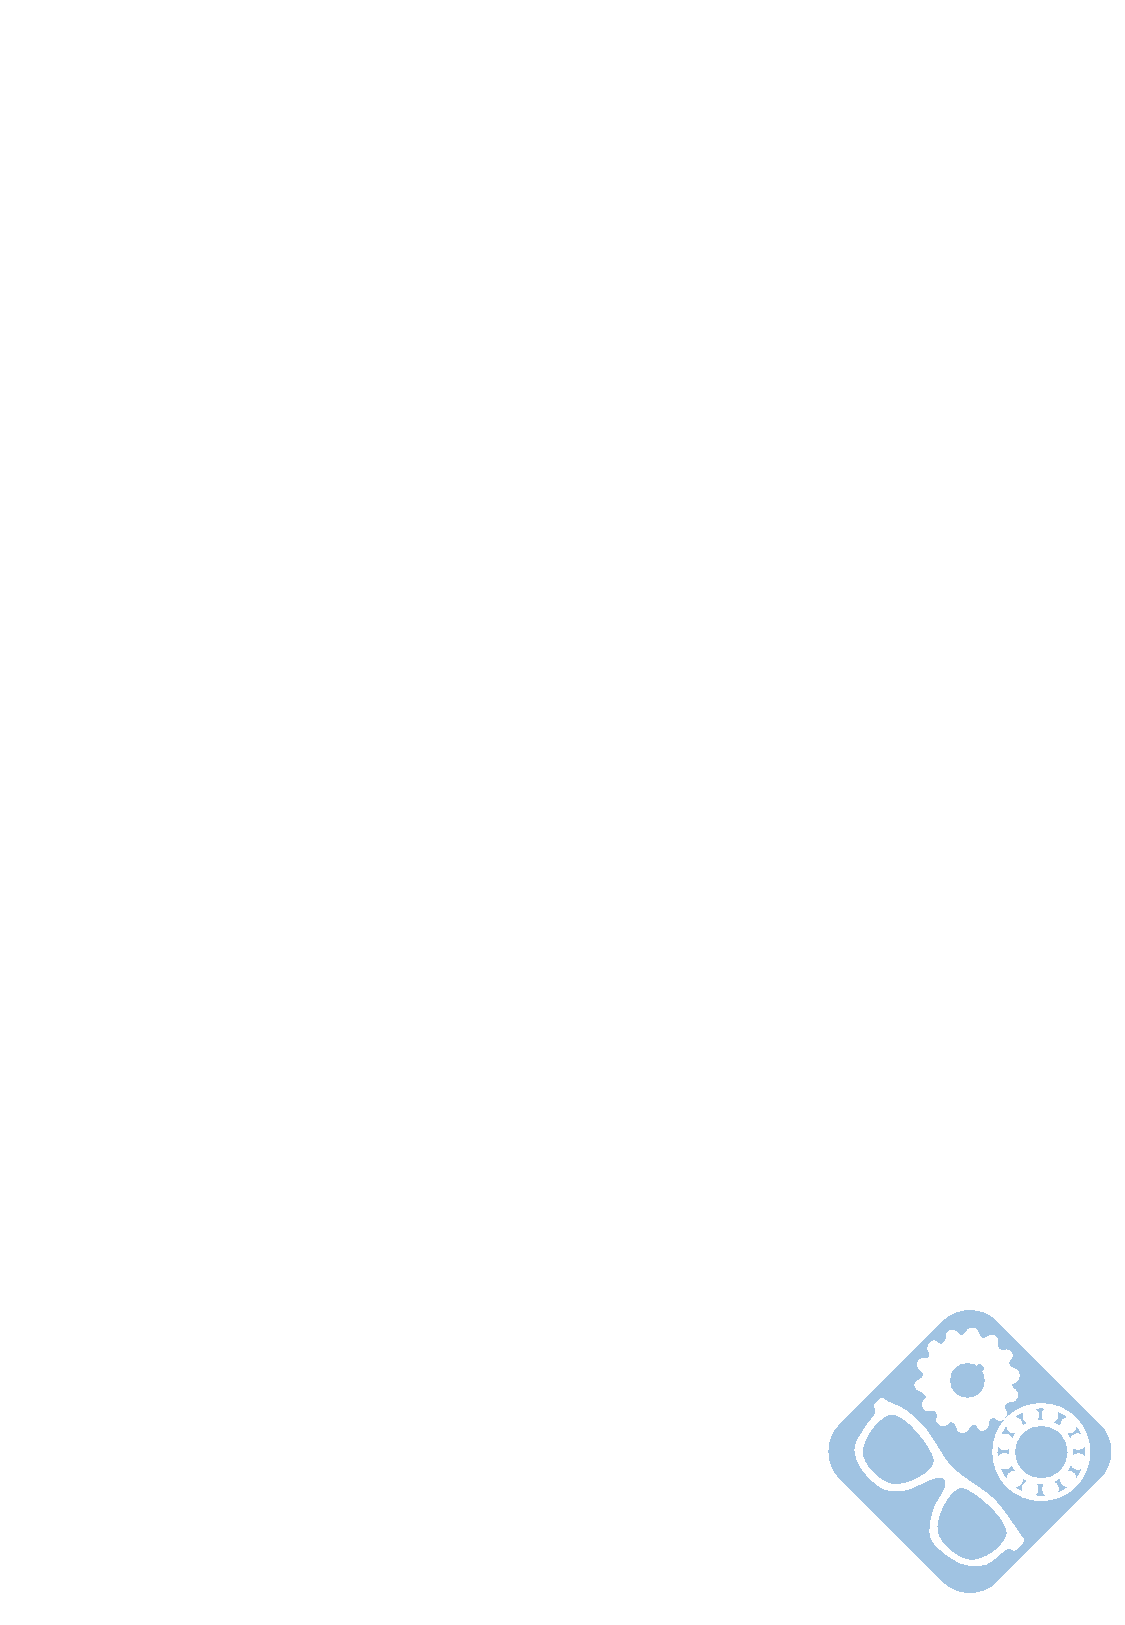
\includegraphics[width=\paperwidth,height=\paperheight,%
keepaspectratio]{../../img/fond4}%
\end{center}
\vfill
}}}

\begin{document}

\pagestyle{empty}

\vspace*{-3\baselineskip}

\AddToShipoutPicture*{\BackgroundPic}

\ifdef{\auteurdeux}{\begin{tabular}{>{\columncolor{gray!00}}m{.3\linewidth} m{.3\linewidth} >{\columncolor{gray!00}}m{.3\linewidth}}
Séquence : \sequence &  \multirow{3}{*}{\hspace{1cm}
\includegraphics[height=1.5cm]{../../img/logo}} &  \begin{flushright} \multirow{4}{*}{\hspace{1cm}\includegraphics[height=4cm]{img/qrcode}}\end{flushright}\\
Document : \type\num \\
 \institute \\
 \auteurun\\
 \auteurdeux
\end{tabular}}{\begin{tabular}{>{\columncolor{gray!00}}m{.3\linewidth} m{.3\linewidth} >{\columncolor{gray!00}}m{.3\linewidth}}
Séquence : \sequence &  \multirow{3}{*}{\hspace{1cm}
\includegraphics[height=1.5cm]{../../img/logo}} &  \begin{flushright} \multirow{4}{*}{\hspace{1cm}\includegraphics[height=4cm]{img/qrcode}}\end{flushright}\\
Document : \type\num \\
 \institute \\
 \auteurun
\end{tabular}}

\vspace{1cm}

\ifdef{\prive}{\begin{center}\colorbox{danger}{\Huge{Avec Correction}}\end{center}}{}

\begin{center}\huge{\nom}\end{center}

\vspace{2cm}

\ifdef{\imagedeux}{\begin{minipage}{0.49\linewidth}}{}
\begin{center}\includegraphics[height=5cm]{/home/renaud/Documents/Renaud/GitHub/django_education/systemes/\imageun}\end{center}
\ifdef{\imagedeux}{\end{minipage}\hfill
\begin{minipage}{0.49\linewidth}
\begin{center}\includegraphics[height=5cm]{/home/renaud/Documents/Renaud/GitHub/django_education/systemes/\imagedeux}\end{center}
\end{minipage}}{}

\vspace{5cm}


\begin{tabular}{p{.15\linewidth} >{\columncolor{white}}p{.8\linewidth}}
    \rowcolor{gray!20}
    Référence & S\sequence\ - \type\num \\
    Compétences & \competences \\
 	\rowcolor{gray!20}
    Description & \descrip \\
    Système & \systemes
  \end{tabular}

\newpage

\AddToShipoutPicture{\BackgroundPicdeux}

\pagestyle{normal}

\section{Tapis de course à pied TC 790}

\subsection{Présentation}

\begin{figure}[!h]
  \begin{minipage}{0.35\linewidth}
  \centering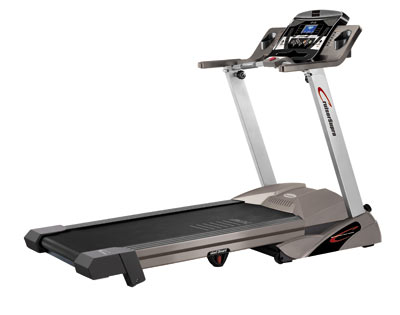
\includegraphics[width=0.8\linewidth]{img/tapis.jpg}
  \caption{Tapis de course}
  \label{img4}
  \end{minipage}
  \hfill
  \begin{minipage}{0.60\linewidth}
Depuis maintenant plusieurs décennies, on constate un essor de la pratique des sports d'extérieur dans les salles de fitness, faisant apparaître régulièrement de nouveaux appareils.

Ainsi, au début des années 1980, des tapis permettant de pratiquer la course à pied à l'instar des vélos d'appartement ou encore des rameurs sont apparus.
\end{minipage}
\end{figure}

\begin{figure}[!h]
  \begin{minipage}{0.3\linewidth}
    \centering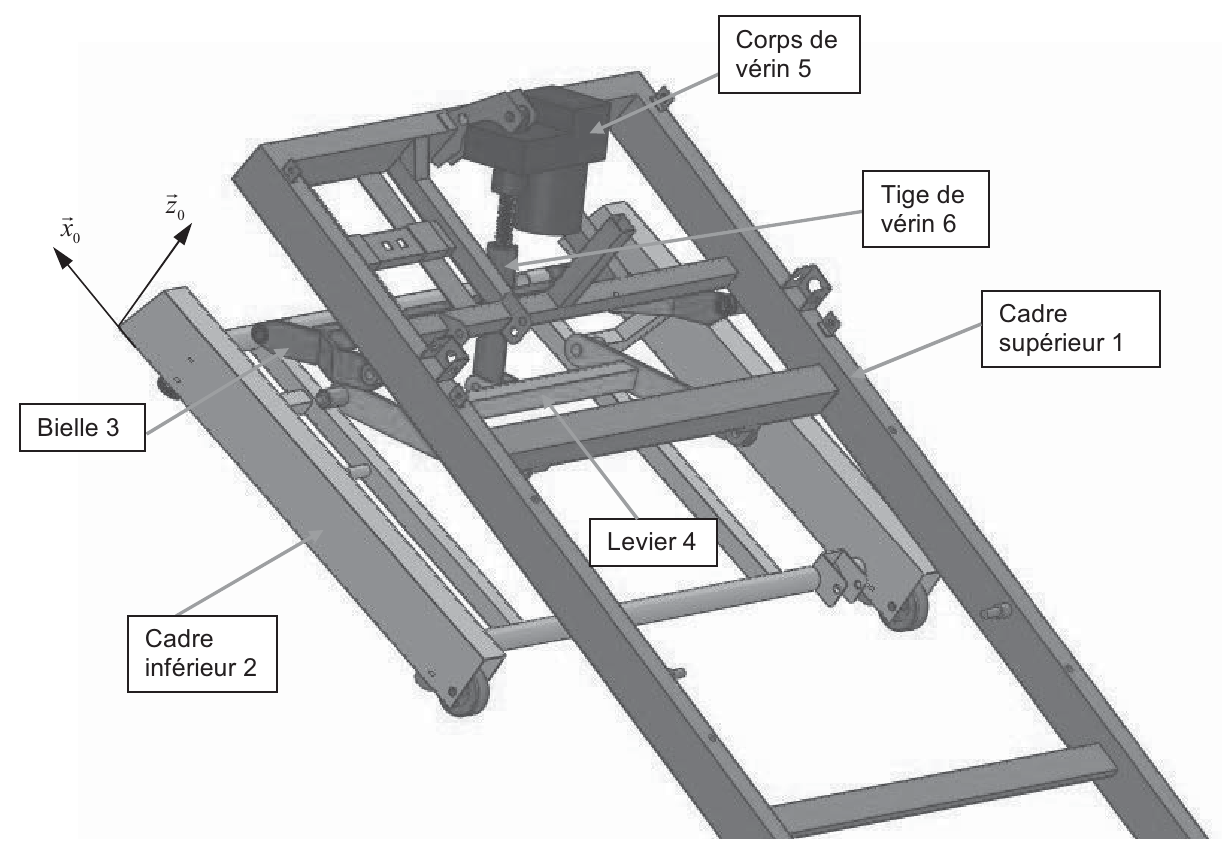
\includegraphics[width=1\linewidth]{img/tapis_reduc.png}
  \end{minipage}
  \hfill
  \begin{minipage}{0.40\linewidth}
    \centering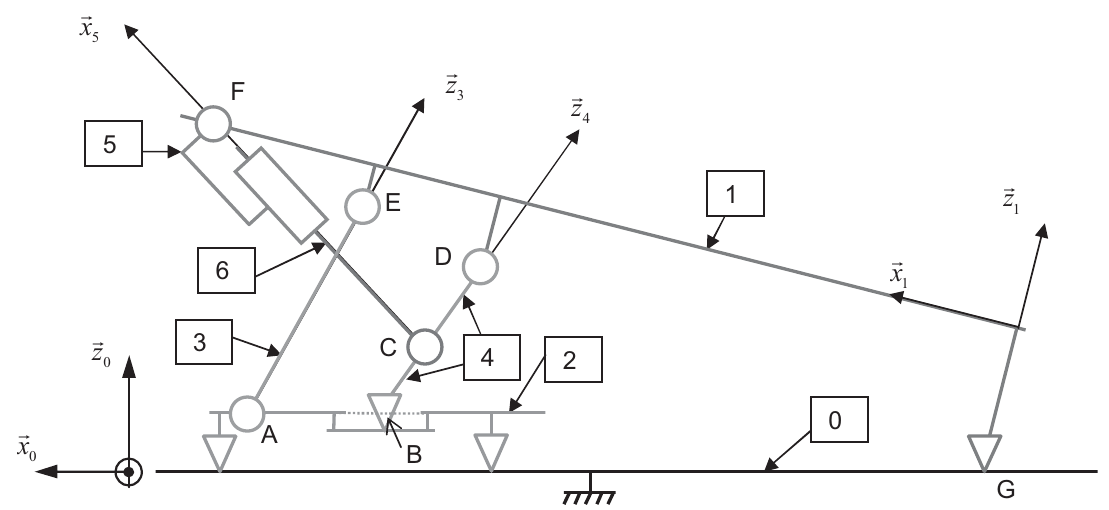
\includegraphics[width=1\linewidth]{img/tapis_cin.png}
  \end{minipage}
  \hfill
  \begin{minipage}{0.27\linewidth}
   \centering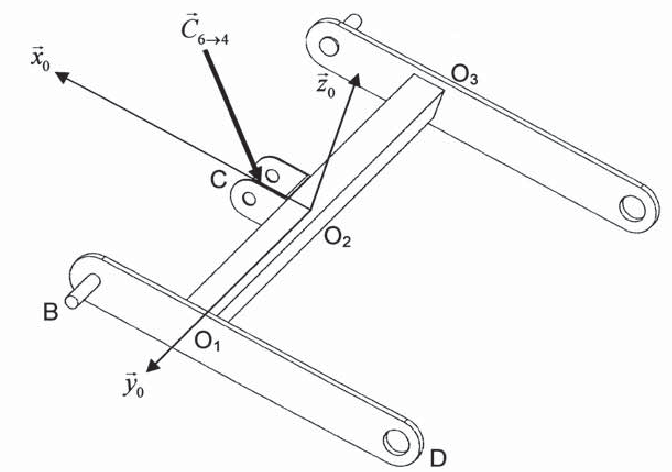
\includegraphics[width=1\linewidth]{img/levier.png}
  \end{minipage}
  \caption{Schéma du tapis}
\end{figure}

\subsection{Étude statique}

L'objectif est de déterminer l'effort maximal que doit développer le vérin afin de maintenir le tapis à l'équilibre. On se contente ici d'une étude dans le domaine statique car l'élévation du tapis se fait à une vitesse quasi-constante et les accélérations mises en jeu sont faibles.

L'étude est faite dans le cas le plus défavorable. On considère le coureur ayant la masse maximum indiquée dans le cahier des charges, c'est-à-dire 130 kg. Il est positionné le plus en avant sur la bande de course. Le cadre est en position horizontale : $\alpha_{10}=0$\textdegree.

L'étude est menée dans le plan. Les glisseurs seront introduits de la façon suivante : en M, pour une liaison entre les solides $i$ et $j$, la résultante d'actions mécaniques est notée $\overrightarrow{M_{i \rightarrow j}}=Z_M.\overrightarrow{z_\alpha}+X_M.\overrightarrow{x_\alpha}$ où $B_\alpha=\left(\overrightarrow{z_\alpha},\overrightarrow{x_\alpha}\right)$ est la base de projection. On pourra également noter ce vecteur $\overrightarrow{M_{i \rightarrow j}}=M_{i \rightarrow j}.\overrightarrow{u_\alpha}$ avec$ \overrightarrow{u_\alpha}$ un vecteur unitaire.

Données :
\begin{itemize}
 \item L'action de pesanteur sur le coureur est notée $\overrightarrow{P_{coureur}}=-P_{coureur}.\overrightarrow{z_0}$ s'appliquant en $G_{coureur}$,
 \item L'action de pesanteur sur le cadre supérieur ainsi que toutes les pièces qu'il supporte est notée $\overrightarrow{P_{cadre}}=-P_{cadre}.\overrightarrow{z_0}$ s'appliquant en Gc ;
 \item On note $\overrightarrow{GG_{coureur}}.\overrightarrow{x_0}=x_{coureur}$ et $\overrightarrow{GG_c}.\overrightarrow{x_0}=x_{cadre}$.
\end{itemize}

Hypothèses:
\begin{itemize}
 \item Toutes les liaisons sont considérées sans frottement,
 \item La pièce 2 sera considérée encastrée avec le sol,
 \item Les poids des autres pièces sont négligés.
\end{itemize}

\paragraph{Question 1:} Vous utiliserez pour répondre la figure \ref{img45}. Déterminer les directions des efforts en A, B, C, D, E et F. Indiquer notamment dans le tableau proposé les isolements successifs réalisés, et pour chaque isolement l'(les) effort(s) pour lequel(lesquels) la direction a été déduite. Réaliser sur la figure proposée la construction graphique associée.

\begin{figure}[!h]
    \centering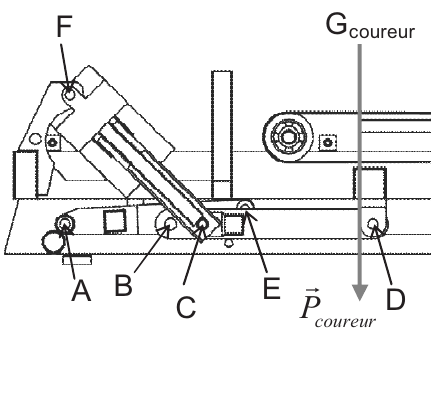
\includegraphics[width=0.5\linewidth]{img/isolement_2.png}

\vspace{1cm}
 
   \centering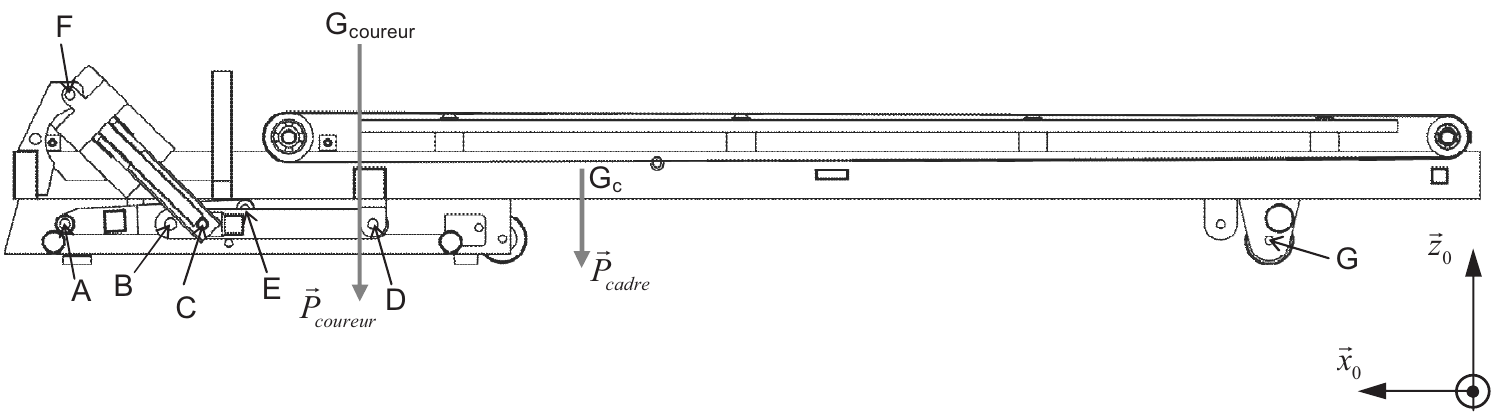
\includegraphics[width=0.8\linewidth]{img/isolement.png}

 \vspace{-1.5cm}
    \caption{Isolement des pièces du tapis}
  \label{img45}
\end{figure}

On note : $\overrightarrow{C_{6 \rightarrow 4}}=Z_C.\overrightarrow{z_0}+X_C.\overrightarrow{x_0}$ l'effort en C et $\overrightarrow{D_{1 \rightarrow 4}}=Z_D.\overrightarrow{z_0}+X_D.\overrightarrow{x_0}$ l'effort en D.

\paragraph{Question 2:} Préciser l'isolement et le théorème utilisé permettant de montrer que $X_C=-X_D$. Cette relation reste-t-elle valable quelque soit l'angle d'inclinaison du cadre supérieur ?

On note : $\overrightarrow{E_{3 \rightarrow 1}}=Z_E.\overrightarrow{z_0}+X_E.\overrightarrow{x_0}$ l'effort en E et $\overrightarrow{F_{1 \rightarrow 5}}=Z_F.\overrightarrow{z_0}+X_F.\overrightarrow{x_0}$ l'effort en F.

\paragraph{Question 3:} Préciser l'isolement et le théorème utilisé permettant de déterminer $X_E$. En déduire l'expression de $\overrightarrow{E_{3 \rightarrow 1}}$.

Pour la suite, dans la position du système, en sachant que:
\begin{itemize}
 \item $\overrightarrow{GF}.\overrightarrow{x_0}>>\overrightarrow{GF}.\overrightarrow{z_0}$
 \item $\overrightarrow{GD}.\overrightarrow{x_0}>>\overrightarrow{GD}.\overrightarrow{z_0}$
\end{itemize}

On supposera 
\begin{itemize}
 \item $\overrightarrow{GF}=x_{GF}\cdot\overrightarrow{x_0}$
 \item $\overrightarrow{GD}=x_{GD}\cdot\overrightarrow{x_0}$
\end{itemize}


\paragraph{Question 4:} Préciser l'isolement et le théorème utilisé permettant de déterminer une relation entre $x_{GF}$, $x_{GD}$, $Z_F$, $Z_D$, $P_{courreur}$, $P_{cadre}$, $x_{coureur}$ et $x_{cadre}$.

\newpage

\section{Robot de consolidation de parois rocheuses: Le \og Roboclimber \fg}

\subsection{Présentation du système}

\begin{figure}[!h]
  \begin{minipage}{0.49\linewidth}
\begin{flushleft}
Roboclimber est un robot géotechnique utilisé pour la consolidation des talus de sols naturels ou des escarpements rocheux au dessus des routes ou des zones habitées. Il est issu d'un programme européen de recherche et est actuellement exploité par la société italienne d'ingénierie D'Appolonia.                                                                                                                                                                                                                                                                                                       \end{flushleft}
  \centering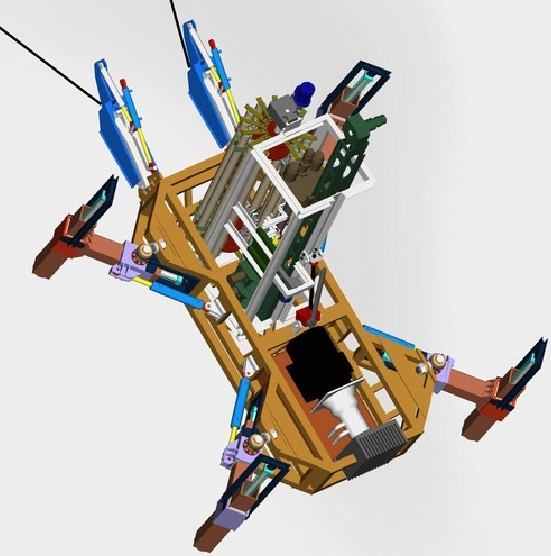
\includegraphics[width=0.7\linewidth]{img/robotclim_sw.png}
  \end{minipage}
  \hfill
  \begin{minipage}{0.49\linewidth}
   \centering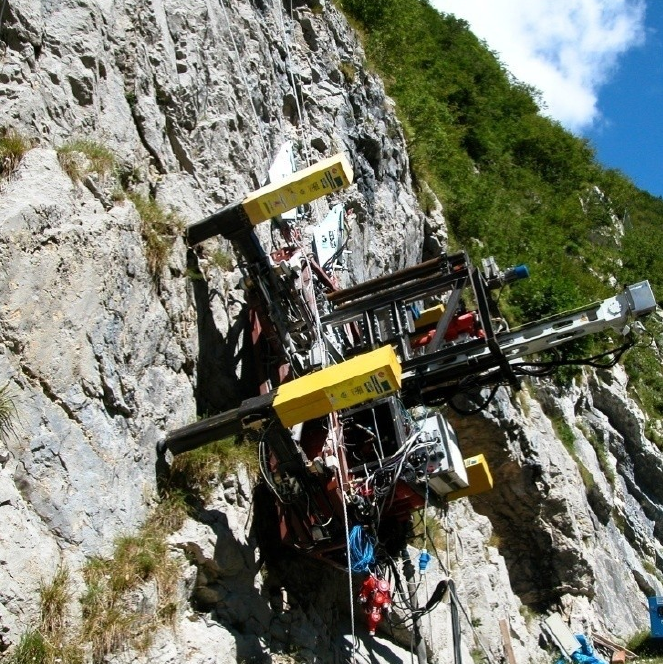
\includegraphics[width=0.7\linewidth]{img/robotclim.png}
   
\begin{flushleft}
   Le Roboclimber est un robot d'environ 3 tonnes transportant une unité autonome de forage et de pose des pieux. Il utilise pour se mouvoir et assurer son équilibre lors du forage 4 pieds indépendants, ainsi que deux câbles de traction fixés en hauteur.\end{flushleft}
  \end{minipage}
  \caption{Roboclimber}
\end{figure}

\subsection{Vérification du critère \og Saisir les tubes \fg}

Un bras automatisé est chargé de déplacer les tubes depuis le carrousel, où ils sont stockés, vers la foreuse où ils seront assemblés au train de tubes. L'effecteur de ce bras est une pince dont on valide ici certains critères fonctionnels.

\textbf{Problématique :} La conception de la pince s'est faite sous la double contrainte de la fiabilité (car le robot est autonome) et de l'encombrement (car la place pour saisir un tube sur le barillet est réduite).

Pour garantir une fiabilité optimale, il a été choisi de ne munir ce dispositif à deux degrés de liberté que d'un seul actionneur : un vérin hydraulique.

Ainsi, le même vérin va assurer le déplacement en translation de la pince, de façon à venir en contact avec le tube, et la fermeture / ouverture des doigts pour la saisie du tube.

Quand la paume est en contact avec le tube, le schéma cinématique de la pince \og doigts ouverts \fg peut être ramené à celui de la figure \ref{roboclimber_cin}.

\newpage

\begin{figure}[h!]
 \centering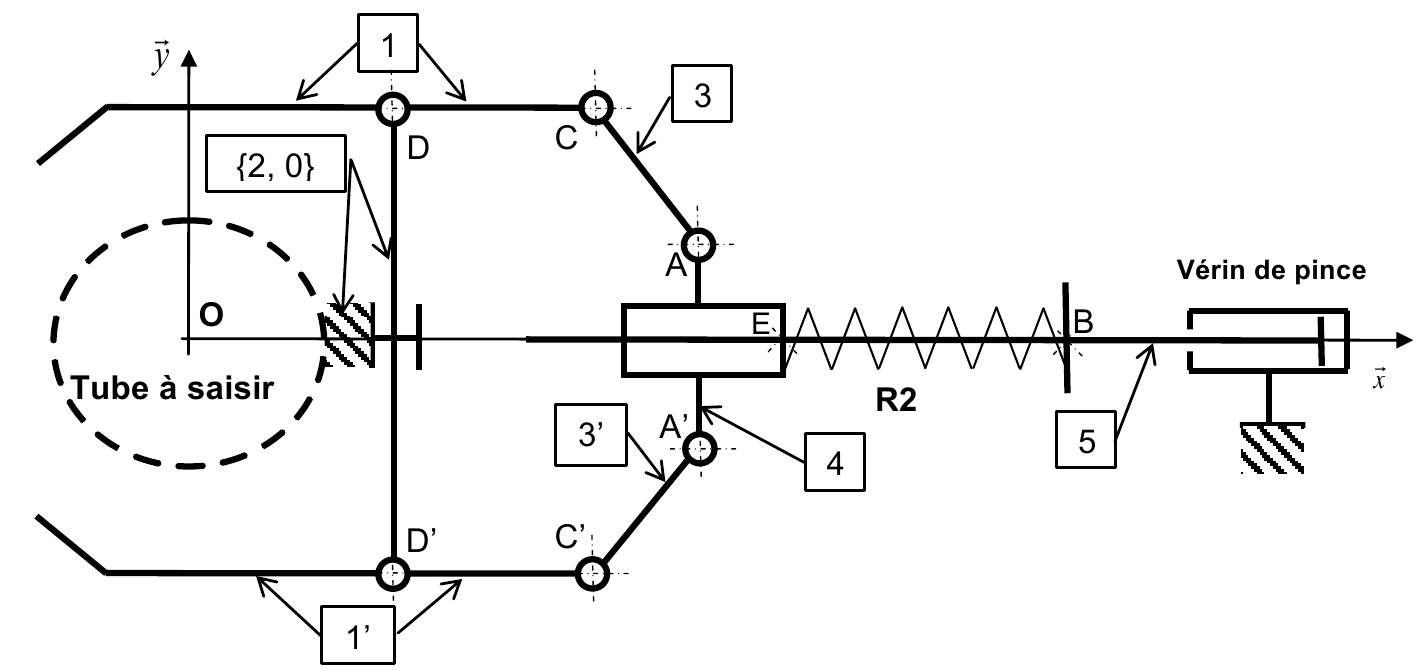
\includegraphics[width=0.9\linewidth]{img/pince_robo_cin.png}
 \caption{Schéma cinématique de la pince}
 \label{roboclimber_cin}
\end{figure}

Lors de la phase d'avance, le ressort R2, de raideur $k_2$ , n'est pas comprimé. On note sa longueur à vide $l_{02}$.

A un instant $t$, on note $x_A$ l'abscisse du point A et $x_B$ l'abscisse du point B.

Les mouvements étant suffisamment lents, on se place dans le cas de l'équilibre statique dans le référentiel lié au corps de la pince supposé galiléen.

\paragraph{Question 1:}

Par des constructions géométriques sur le dessin du document-réponse, déterminer le déplacement $\Delta x_A$ du point A de la position \og paume en contact avec le tube \fg à la position \og doigts fermés \fg.

A partir de cette position \og pince fermée \fg (dans laquelle le ressort R2 n'est pas encore comprimé), la tige du vérin est sortie d'une longueur supplémentaire $|\Delta x_B|$ $\left(\Delta x_B <0\right)$, qui provoque l'effort de verrouillage des doigts sur le tube en exerçant un effort sur le coulisseau 4 décrit par le glisseur :
$\left\{R_{2 \rightarrow 4}\right\}=\left\{
\begin{array}{c}
 k_2.\Delta x_B.\overrightarrow{x} \\
 \overrightarrow{0}
\end{array}\right\}_E$

On fixe $\Delta x_B=-31mm$, on donne $k_2=13N.mm^{-1}$.

On se place dans le cas de l'équilibre statique dans le référentiel lié au corps de la pince supposé galiléen.

On considère le problème plan et le contact doigt / tube réduit à un point.

Le poids des pièces de la pince est négligé et les liaisons articulations sont sans frottement.

\paragraph{Question 2:}

Par une construction graphique sur le document-réponse, qui sera justifiée, déterminer la force exercée par chaque doigt sur le tube. On considère qu'aucune action extérieure n'est exercée sur le tube et que pour des raisons de symétrie, les forces de contact paume/tube et doigt/tube passent par le centre du tube.

\includepdf[pages=3-4]{img/roboclimber_dr.pdf}

\newpage

\section{L'attelage automatique Type 10L}

\subsection{Présentation du système}

\begin{figure}[!h]
  \begin{minipage}{0.35\linewidth}
  \centering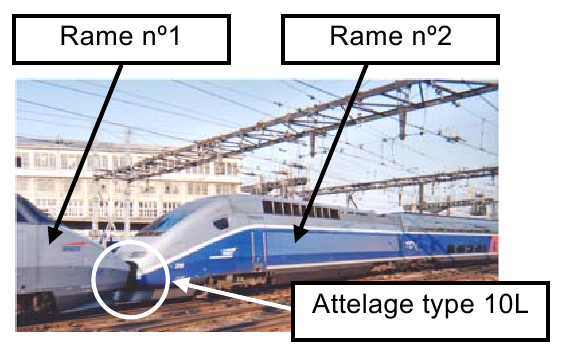
\includegraphics[width=1\linewidth]{img/tgv.png}
  \end{minipage}
  \hfill
  \begin{minipage}{0.60\linewidth}
Pour offrir aux passagers des déplacements à très grande vitesse, la SNCF dispose de rames TGV composées chacune de 2 motrices encadrant 8 voitures.

Dans certains cas d'affluence, veille de « grand week-end » ou vacances scolaires, afin de transporter un maximum de passagers, la SNCF réalise l'assemblage de 2 rames, au niveau des motrices, par le biais d'un attelage de type 10L. Cet attelage est composé de deux demi-attelages.

Au désaccouplement, il reste un demi-attelage sur chacune des motrices.
  \end{minipage}
  \caption{Attelage TGV}
\end{figure}

\subsection{Problématique de l'étude}

Validation de la fonction \og empêcher les ressorts de compression de se détendre \fg. Dans cette partie, on étudie le mécanisme dans la phase d'approche des deux coupleurs (voir figure 1 du document DT3). Le verrou 3 et la manille 2 sont immobiles par rapport au corps 1, le cliquet 4 n'est pas libéré. 

Pour empêcher les ressorts de compression 10 et 11 de se détendre, la dent du cliquet 4, repérée \og d \fg sur les documents DT4 et DT5, est soumise à un effort de contact important. 

\textbf{Objectif de l'étude :} la surface de contact entre la dent \og d \fg du cliquet 4 et le bossage du corps 6 est restreinte et soumise à une pression importante. La pression superficielle de contact maximale admise, dans ces conditions, est de 50 MPa. On se propose de comparer la pression effective à cette pression admissible afin de valider ou non la dimension de la surface de contact. 

Pour obtenir le résultat recherché, il est nécessaire d'étudier successivement : 
\begin{itemize}
 \item l'équilibre du cylindre d'accouplement $\left\{5,9,10,11\right\}$, 
 \item l'équilibre de la manille $2$, 
 \item l'équilibre du verrou $3$, 
 \item l'équilibre du cliquet $4$. 
\end{itemize}


Hypothèses :
\begin{itemize}
 \item le problème est considéré comme plan dans le plan $\left(O,\overrightarrow{x},\overrightarrow{y}\right)$ dans la position de la coupe B-B du document DT5, 
 \item les liaisons pivots de centres O, A, B, C et F sont considérées comme parfaites (voir DR4), 
 \item le centre F de la liaison pivot entre le cliquet 4 et le verrou 3 est ramené dans ce plan $\left(O,\overrightarrow{x},\overrightarrow{y}\right)$, 
 \item la liaison au point E entre le corps 1 et la manille 2 est considérée comme parfaite, 
 \item la liaison au point H entre la dent du cliquet 4 et le corps 6 est assimilée à une ponctuelle de normale $\left(H,\overrightarrow{y}\right)$, il n'existe pas d'autre liaison entre 4 et 6 et l'action du ressort de pression 7 est négligée, 
 \item les poids des différentes pièces sont négligés devant les autres actions mécaniques, 
 \item l'action des ressorts 10 et 11 sur le piston 5 donne une action mécanique de 5 sur la manille 2 telle que $\|\overrightarrow{B_{5 \rightarrow 2}}\|= 2500 N$. 
\end{itemize}

Les tracés seront effectués sur le document DR4. Les bilans, les justifications et les calculs seront rédigés sur feuille de copie. 

\paragraph{Question 1:} Étudier l'équilibre du cliquet 4 et justifier que le support des actions mécaniques extérieures appliquées est la droite passant par les points H et F (voir DR4, figure 1). 

On prendra $\|\overrightarrow{A_{2 \rightarrow 3}}\|= 2500 N$. $\overrightarrow{A_{2 \rightarrow 3}}$ est représentée sur le document DR4. 

\paragraph{Question 2:} Étudier l'équilibre du verrou 3 en faisant le bilan des actions et déterminer graphiquement, sur la figure 2 du document DR4, les actions mécaniques agissant sur le verrou 3.  

\paragraph{Question 3:} Représenter sur la figure 1 du document DR4, en les désignant, les actions mécaniques extérieures agissant sur le cliquet 4 et indiquer la valeur de leurs normes. 

\paragraph{Question 4:} En réalité le contact en H n'est pas ponctuel mais surfacique. Sachant que l'aire de la surface de contact entre la dent du cliquet 4 et le bossage du corps 6 est de $75 mm^2$, calculer la pression de contact supposée uniforme.

\paragraph{Question 5:} La pression superficielle admissible étant de $50 MPa$, conclure quant à la validité de la dimension de la surface de contact. Justifier votre réponse. 

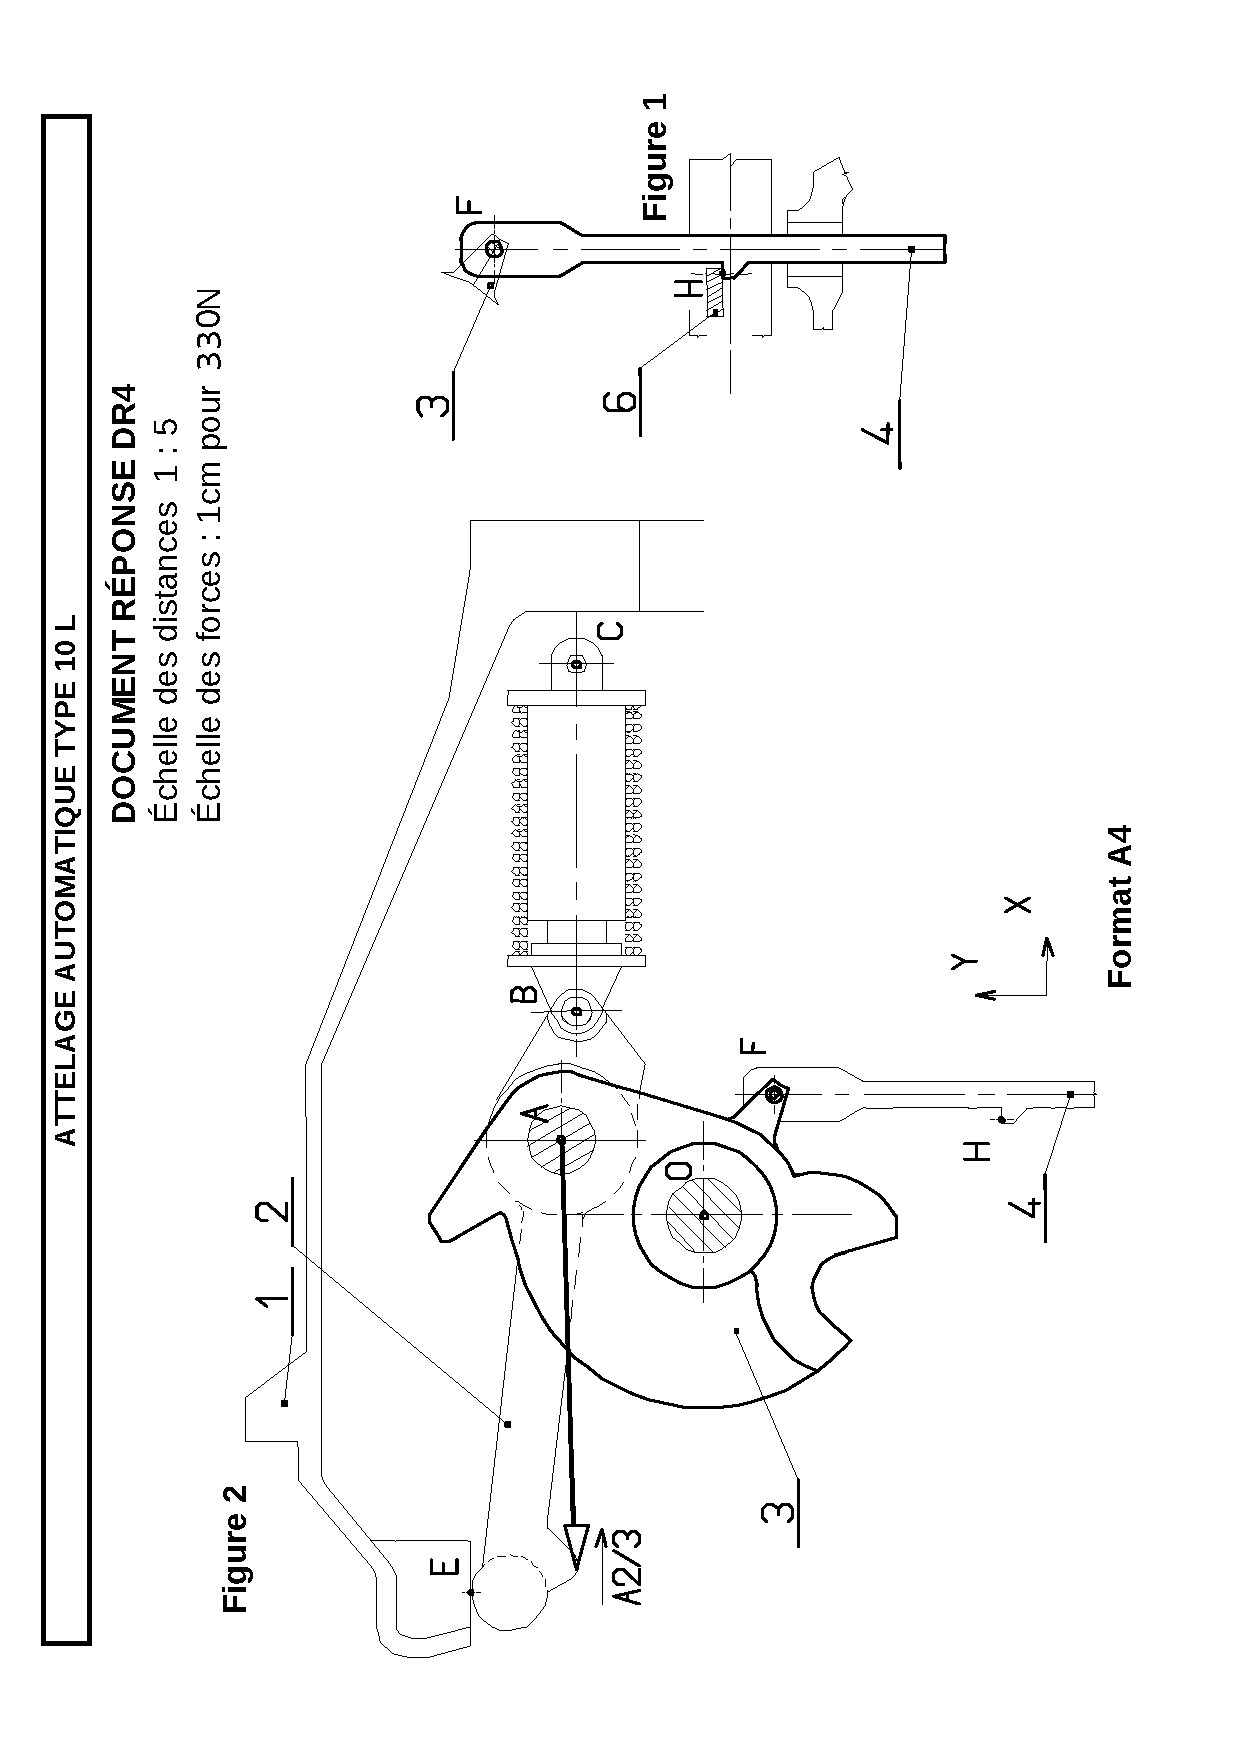
\includepdf{img/tgv.pdf}

\includepdf[pages=23]{img/tgv2.pdf}

\ifdef{\public}{\end{document}}{}

\clearpage

\pagestyle{correction}

\newpage

\section{Correction}

\subsection{Tapis de course à pied TC 790}

\paragraph{Question 1:}

\begin{center}
 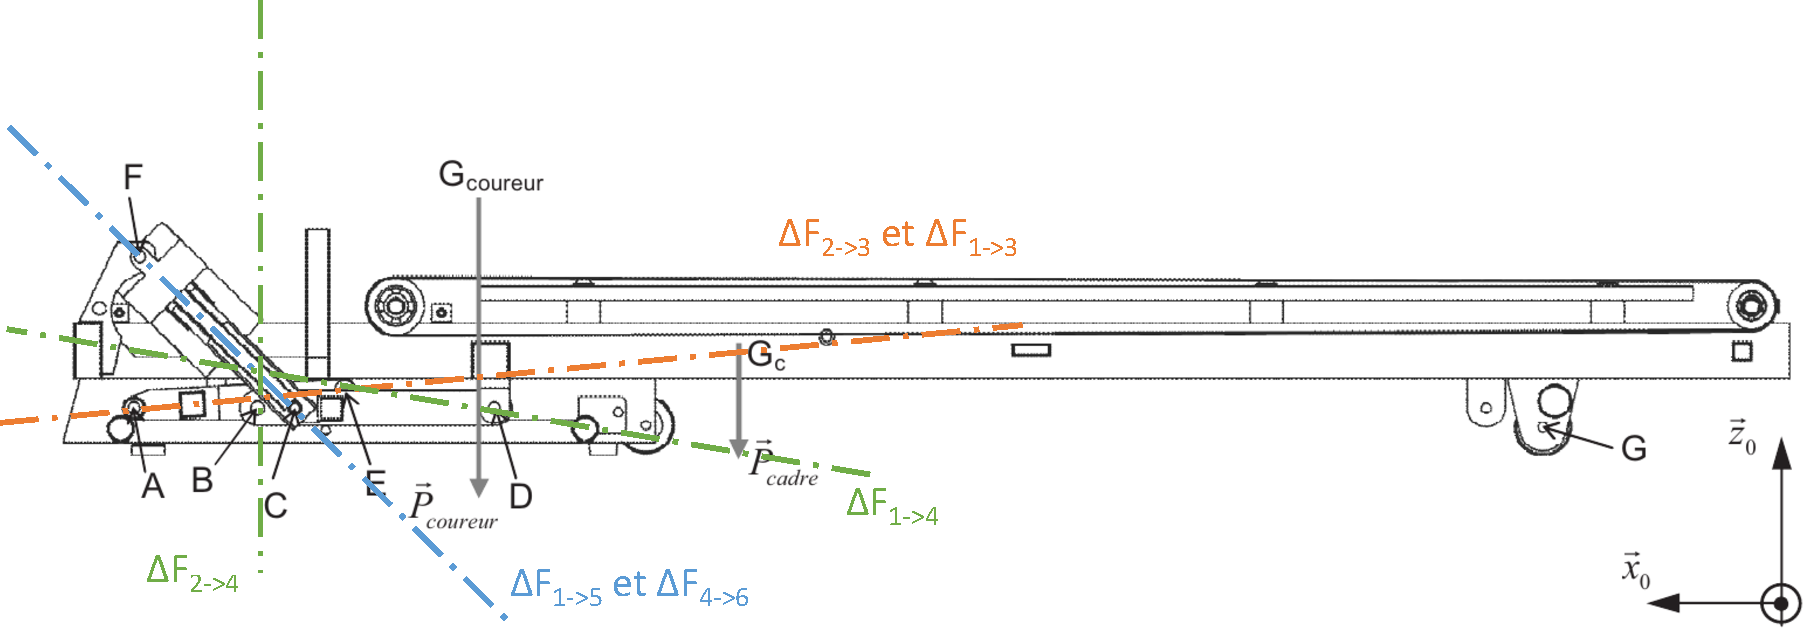
\includegraphics[width=0.9\linewidth]{img/tapis_cor1} \\
 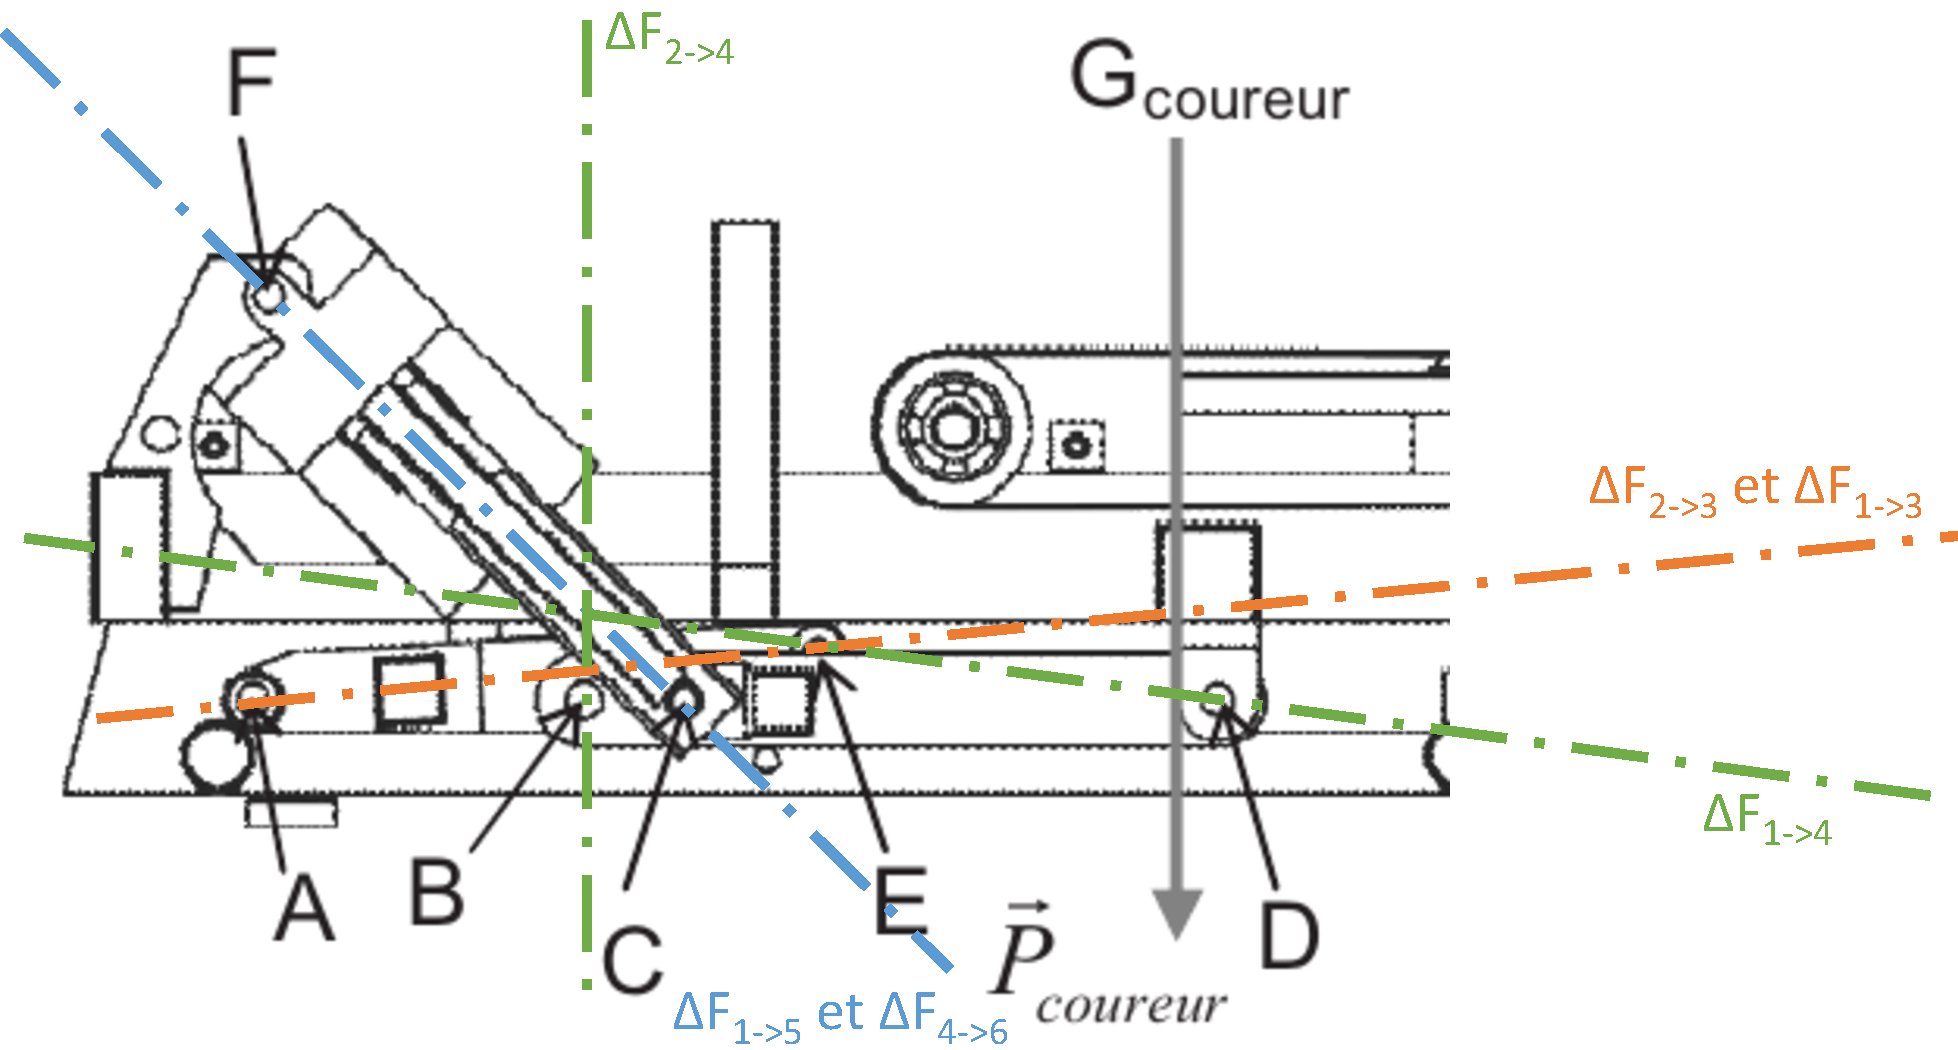
\includegraphics[width=0.6\linewidth]{img/tapis_cor2}
\end{center}

\begin{itemize}
\item 5 + 6 \\
$\overrightarrow{F_{1\rightarrow 5}}$ et $\overrightarrow{F_{4\rightarrow 6}}$ suivant la droite (CF) (Ensemble soumis à 2 forces) \\
\item 3 \\
$\overrightarrow{F_{2\rightarrow 3}}$ et $\overrightarrow{F_{1\rightarrow 3}}$ suivant la droite (AE) (Ensemble soumis à 2 forces) \\
\item 4 \\
La pièce 4 est soumise à 3 forces ($\overrightarrow{F_{6\rightarrow 4}}$, $\overrightarrow{F_{0\rightarrow 4}}$ et $\overrightarrow{F_{1\rightarrow 4}}$). La direction des deux premières est connue (la direction de l'effort en B est verticale car la liaison est une linéaire rectiligne) elles sont coplanaires et concourantes. La direction de l'effort en D passe par le point d'intersection des deux autres.
\end{itemize}

\paragraph{Question 2:}

\begin{itemize}
 \item Solide isolé : La pièce $4$,
 \item Théorèmes utilisé(s) : Théorème de la résultante statique en projection sur l'axe $\overrightarrow{x}$: $X_C+X_D=0$, donc $X_C=-X_D$.
\end{itemize}

Cette relation reste vraie quelle que soit l'inclinaison.

\paragraph{Question 3:}

\begin{itemize}
 \item Solide isolé : L'ensemble $\left\{1,5,6 \right\}$,
 \item Théorème de la résultante statique appliqué à cet ensemble en projection sur l'axe $\overrightarrow{x}$: $X_C+X_D+X_E=0$.
\end{itemize}

D'après la question 11, $X_C+X_D=0$, donc $X_E=0$. La direction de l'effort en E, n'étant pas verticale (droite AE), si $X_E=0$, alors $Z_E=0$, donc $\overrightarrow{E_{3\rightarrow 1}}=\overrightarrow{0}$.

\paragraph{Question 4:}

\begin{itemize}
 \item Solide isolé : La pièce $1$,
 \item Théorème du moment statique appliqué à cet ensemble en projection sur l'axe $\overrightarrow{y_0}$ au point G.
\end{itemize}

$\overrightarrow{M_{G,5\to 1}}=\overrightarrow{M_{F,5\to 1}}+\overrightarrow{GF}\wedge\overrightarrow{F_{5\to 1}}=x_{GF}\overrightarrow{x_0}\wedge(-X_{F}\overrightarrow{x_0}-Z_{F}\overrightarrow{z_0})=x_{GF}~Z_{F}\overrightarrow{y_0}$

De même,
\begin{itemize}
 \item $\overrightarrow{M_{G,4\to 1}}=x_{GD}~Z_{D}\overrightarrow{y_0}$
 \item $\overrightarrow{M_{G,P_{coureur}\to 1}}=x_{coureur}~P_{coureur}\overrightarrow{y_0}$
 \item $\overrightarrow{M_{G,P_{cadre}\to 1}}=x_{cadre}~P_{cadre}\overrightarrow{y_0}$
\end{itemize}

Ainsi, $x_{GF}~Z_{F}+x_{GD}~Z_{D}+x_{coureur}~P_{coureur}+x_{cadre}~P_{cadre}=0$

\newpage

\subsection{Robot de consolidation de parois rocheuses: Le \og Roboclimber \fg}

~\

\begin{center}
 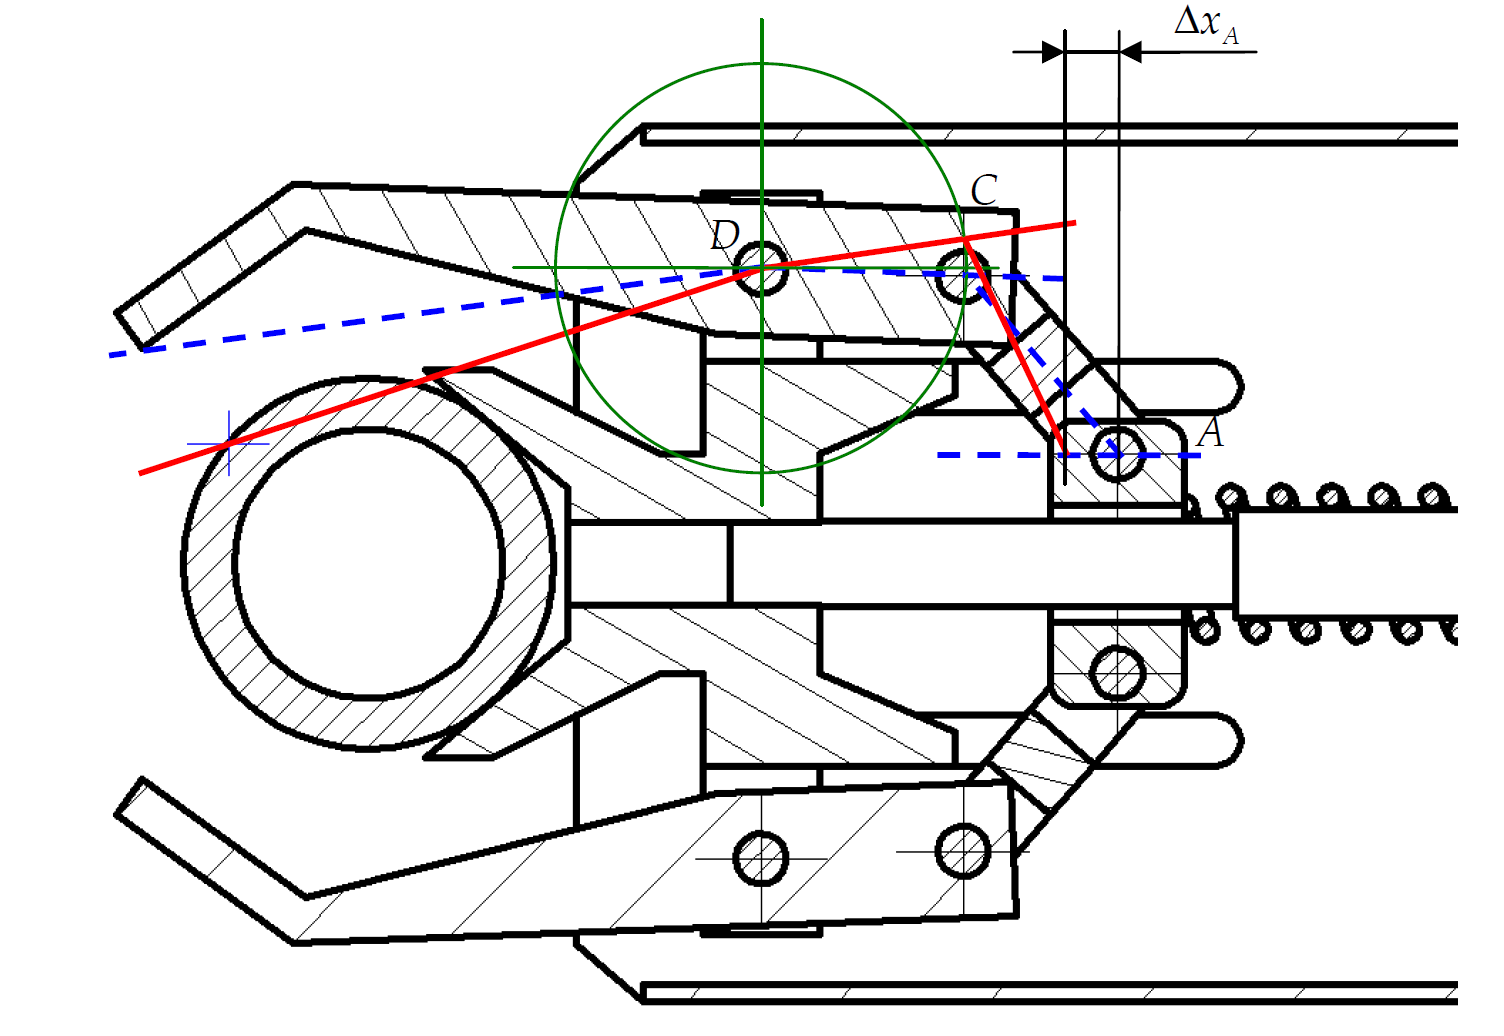
\includegraphics[width=0.8\linewidth]{img/climb1_cor}
\end{center}
 
\begin{center}
 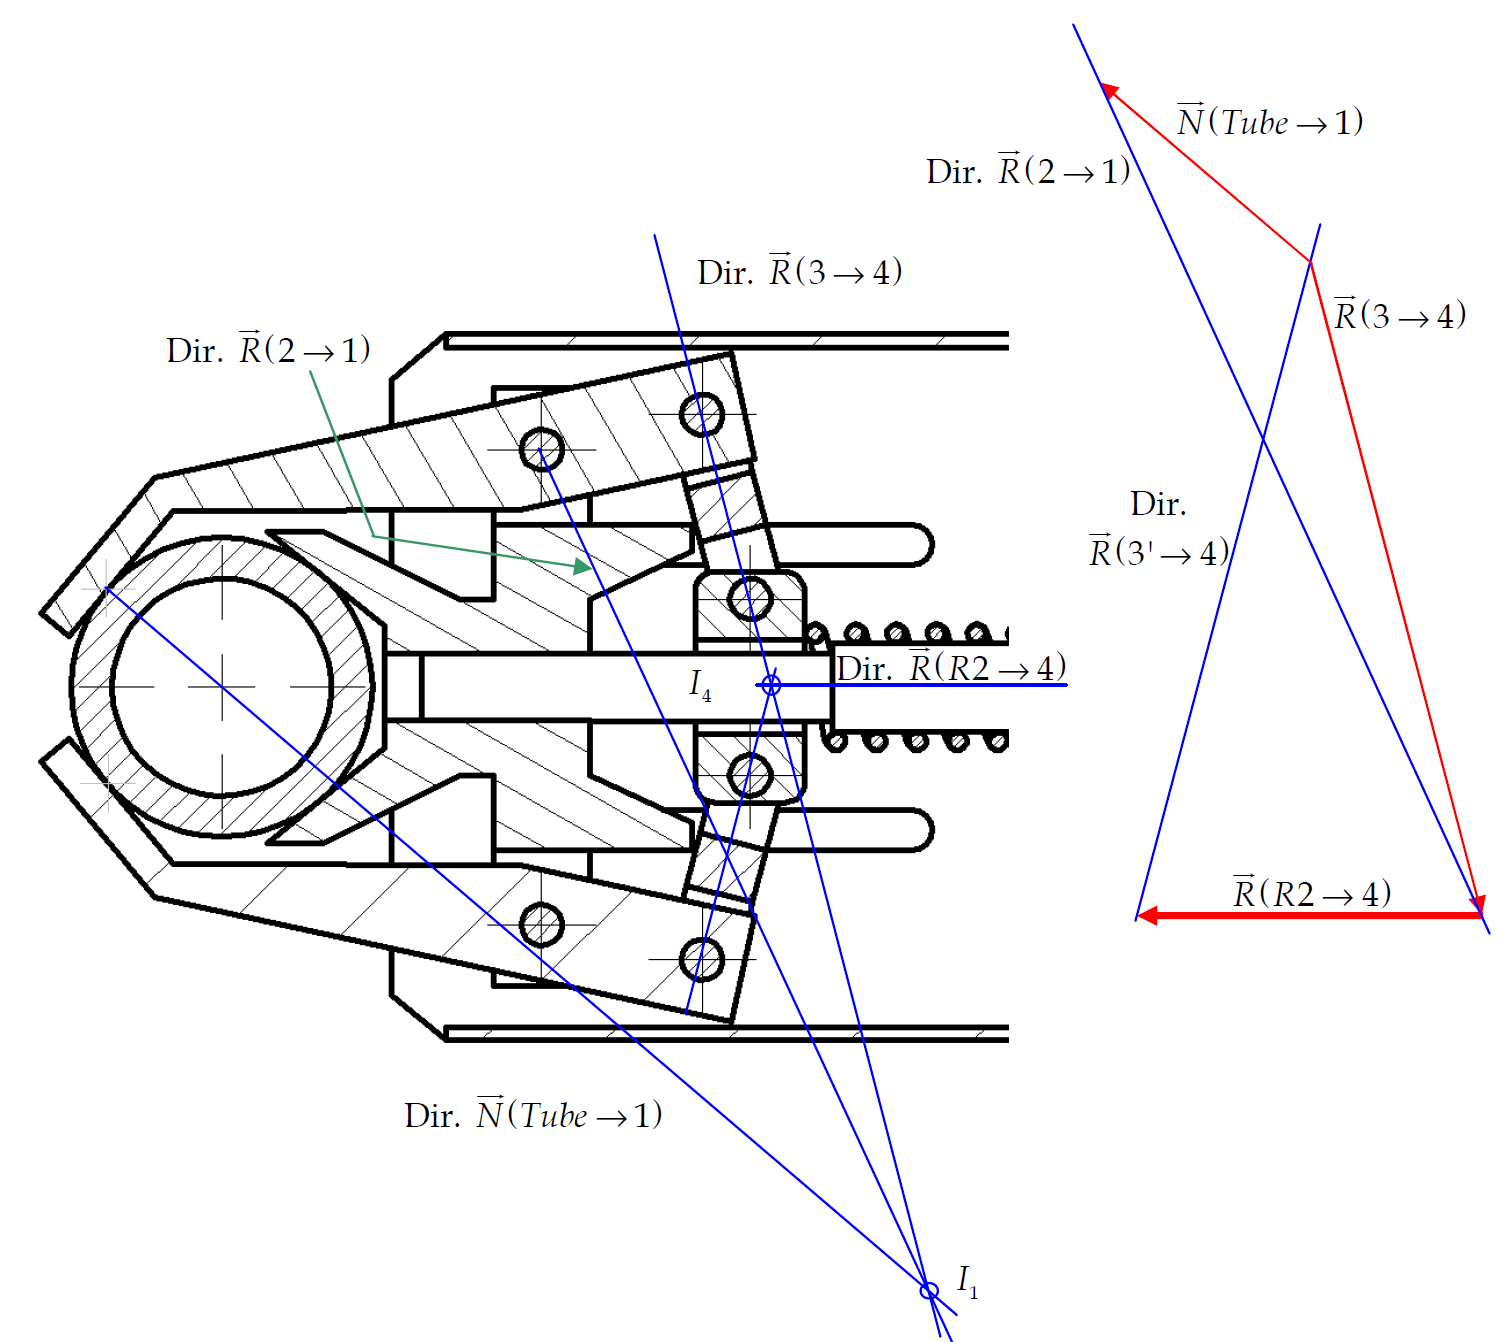
\includegraphics[width=0.9\linewidth]{img/climb2_cor}
\end{center}

\newpage

\subsection{L'attelage automatique Type 10L}

~\

\begin{center}
 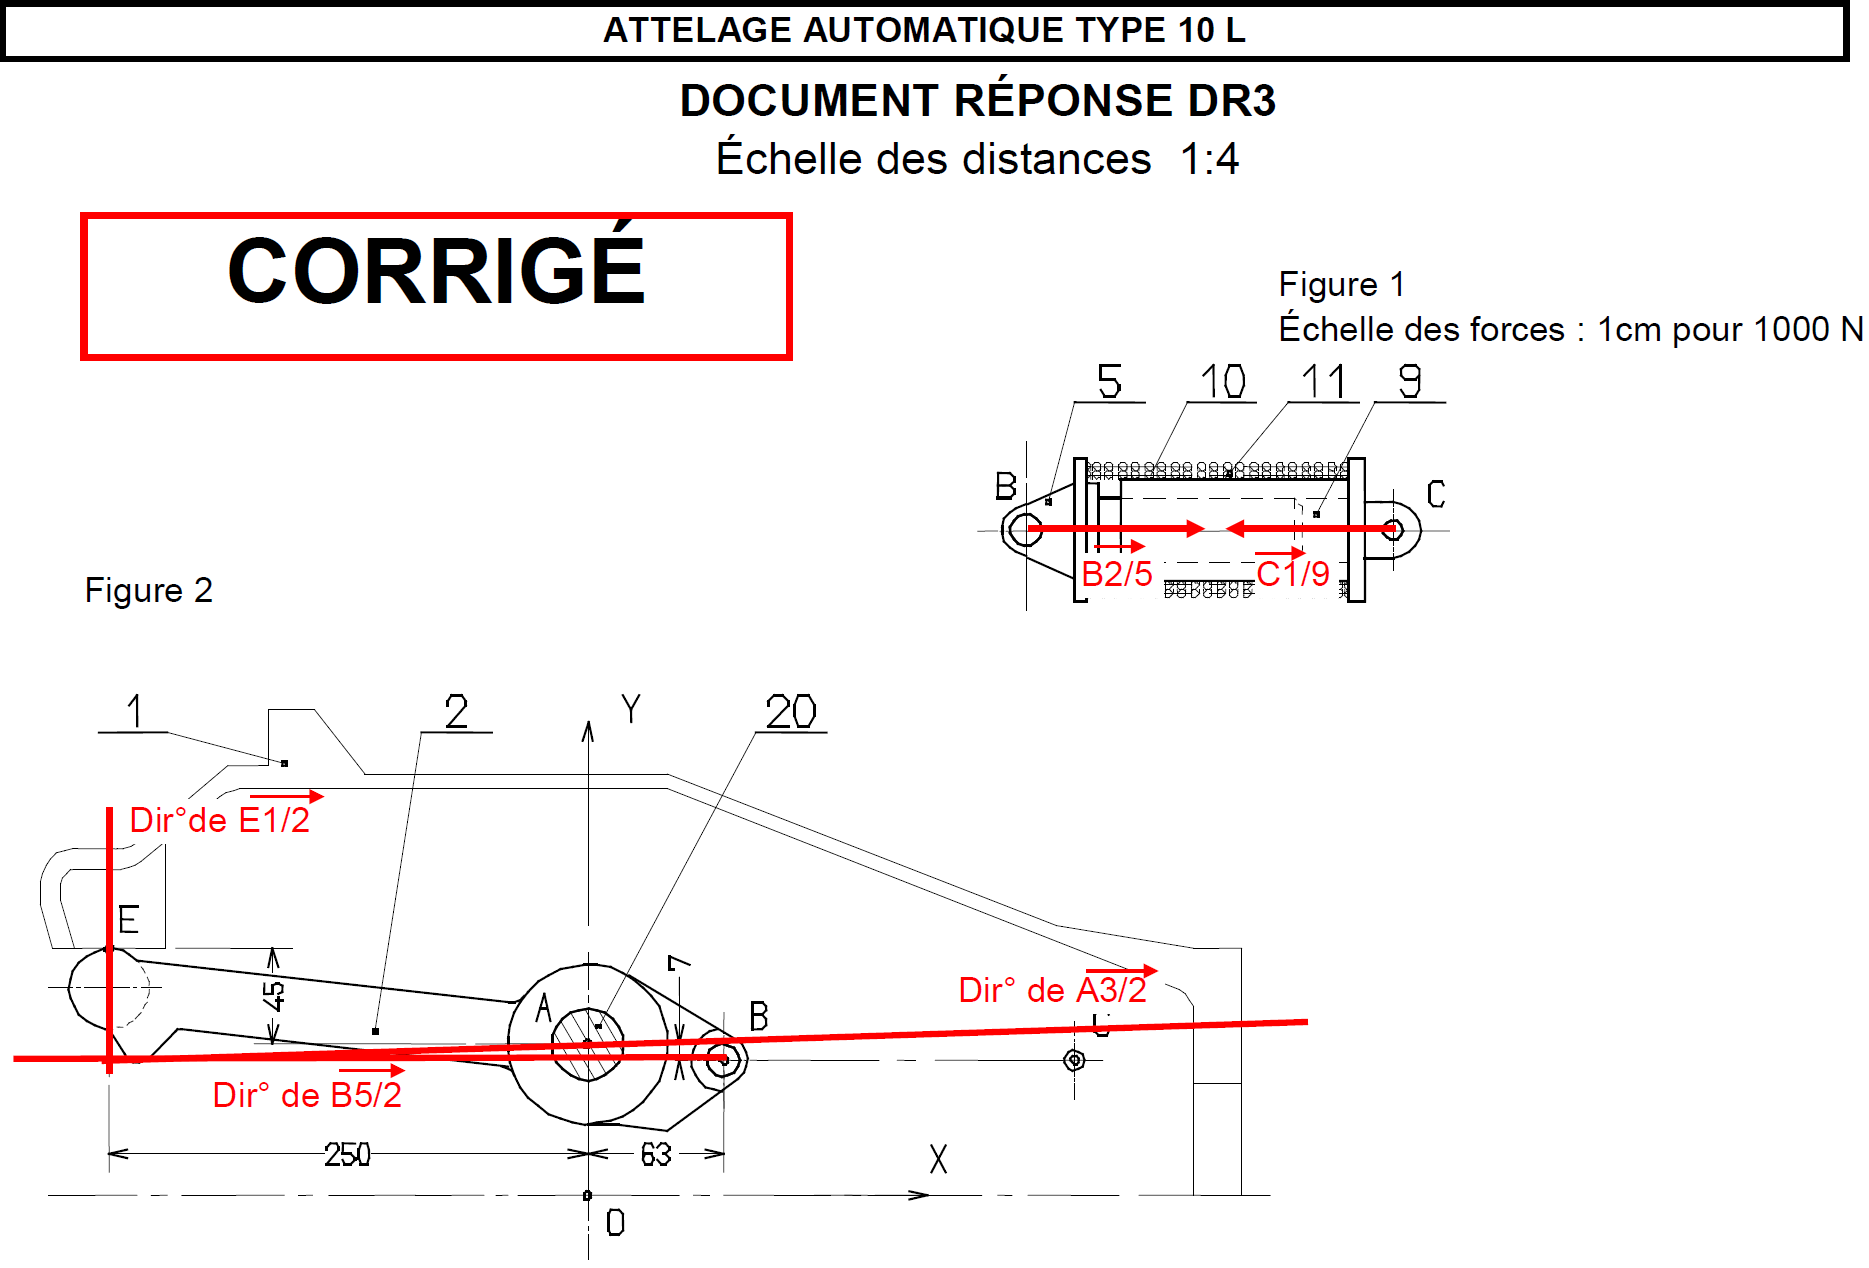
\includegraphics[width=0.9\linewidth]{img/tgv1_cor}
\end{center}
 
\begin{center}
 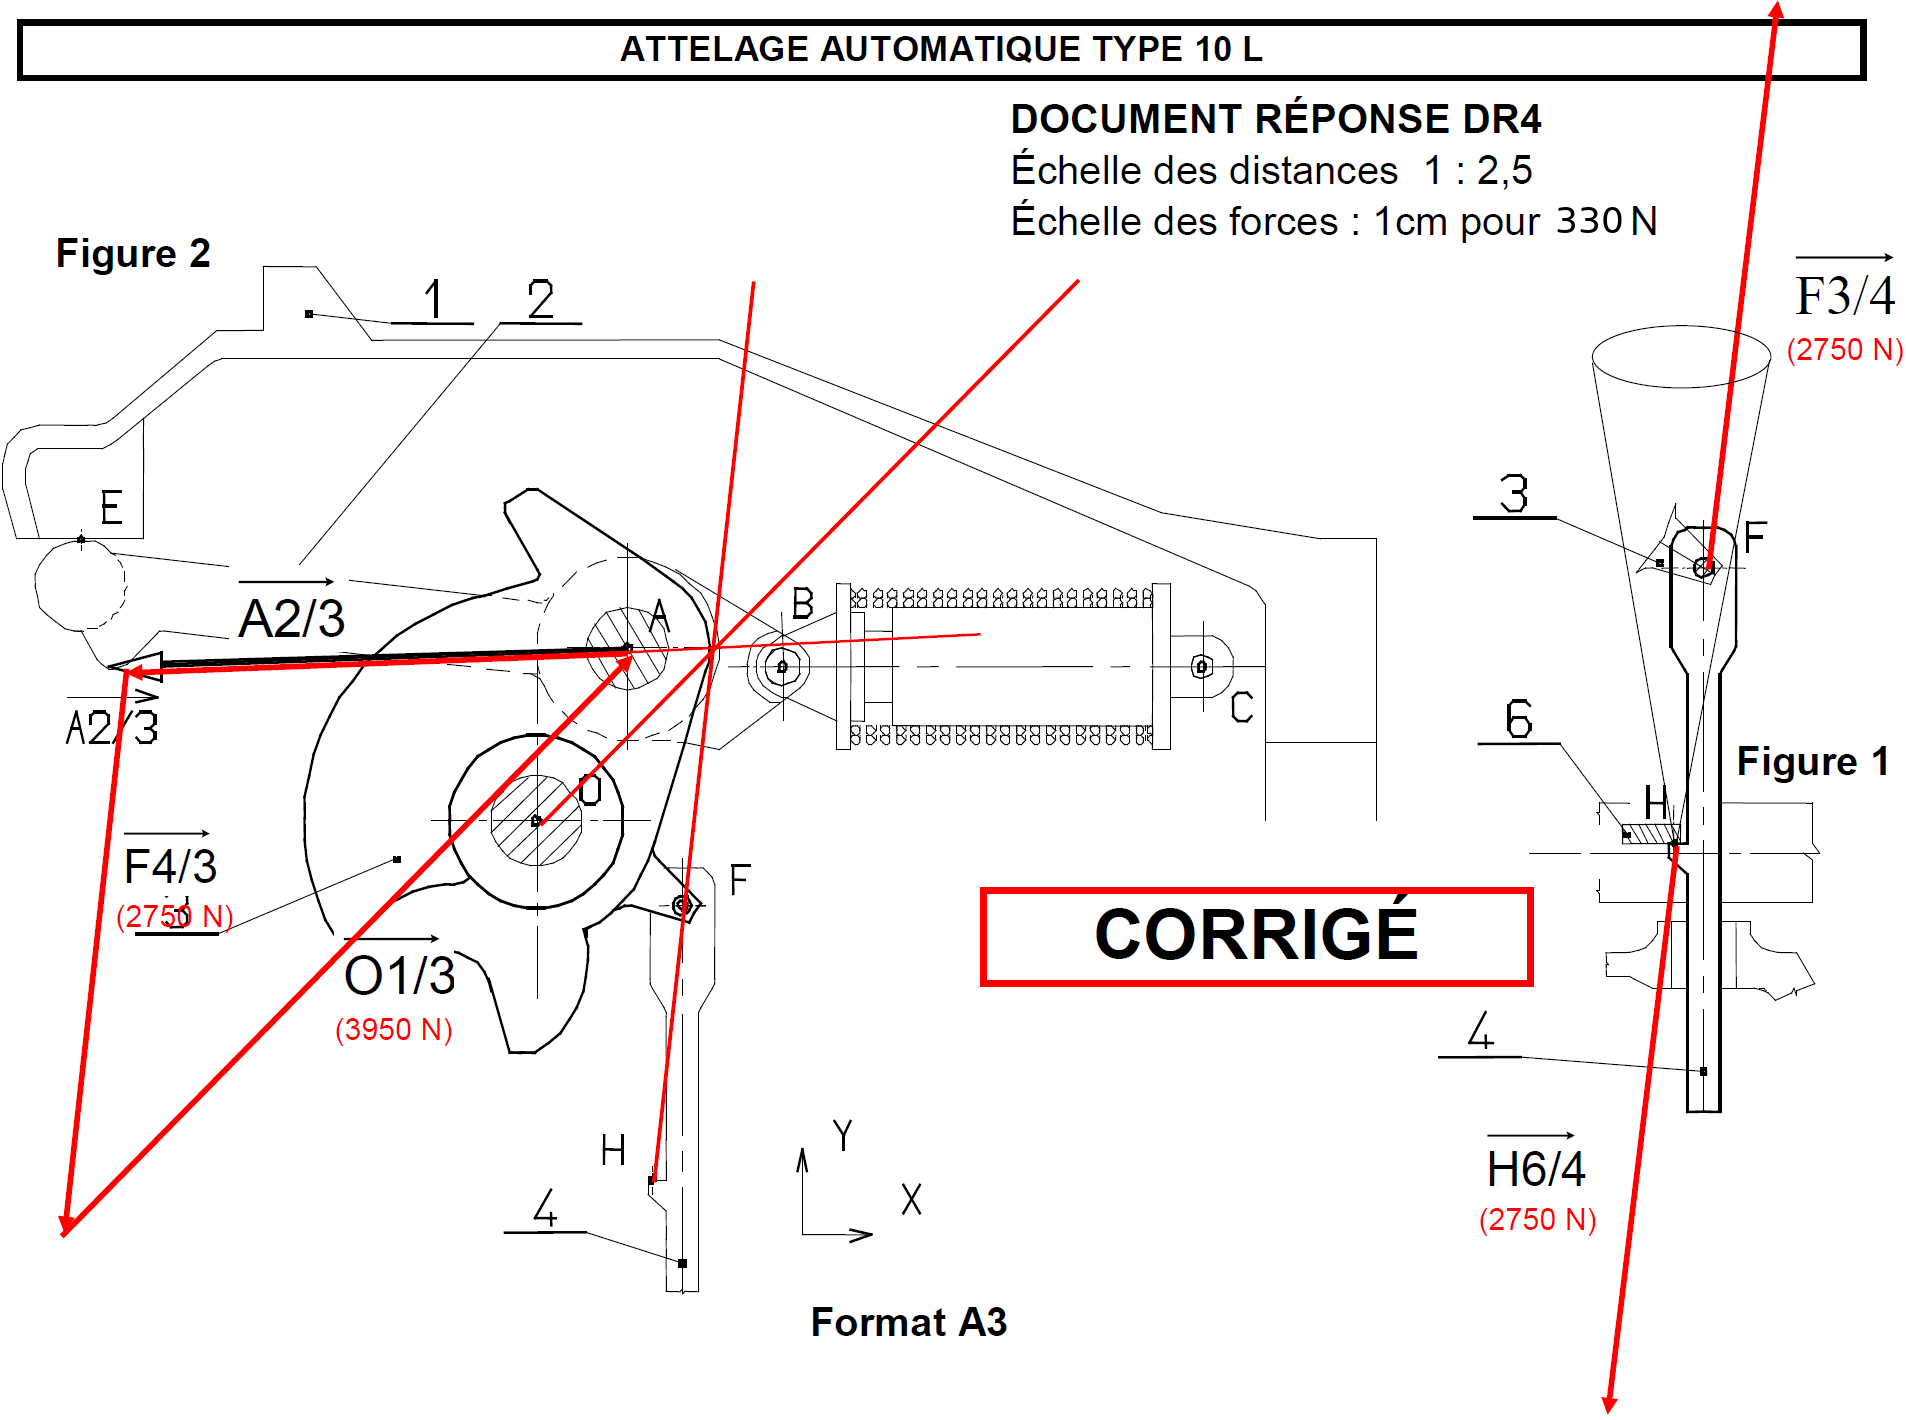
\includegraphics[width=0.9\linewidth]{img/tgv2_cor}
\end{center}

\end{document}